\documentclass[en]{../../../eplsummary}
\usepackage{listings}
\usepackage{float}
\usepackage{graphicx}
\hypertitle{embedded-INGI2146}{8}{INGI}{2146}
{Gorby Nicolas Kabasele Ndonda\and Author2\and Author3}
{Professor}

\section{Introduction}
\begin{description}
    \item[Mobile:] Portable devices with wireless communication,
        running stand-alone or client applications.
    \item[Embedded:] An embedded system is a computer system with
        a dedicated function within a larger mechanical or electrical system.
\end{description}

Embedded systems are everywhere in smartphones, cars,\ldots Typical
characteristics is the following:
\begin{itemize}
    \item Cheap
    \item Reduced power consumption
    \item Real-time
    \item Robust
\end{itemize}

To achieve these characteristic, there need to be a tight coupling between
the hardware, the OS and the application.

\subsection{Real-Time Systems}

Real-Time Systems monitor and have an impact on the physical world via sensors
and actuators. Because of their nature, they have
requirements/constraints on timing:

\begin{description}
    \item[Hard constraint]
        \begin{itemize}
            \item Potentially severe consequences if reaction/result is produced after
                deadline.
            \item Results has no value (or even negative value) after deadline
        \end{itemize}
    \item[Firm constraint]
        \begin{itemize}
            \item Occasional miss tolerated, but degrades QoS
            \item No or little value after deadline
        \end{itemize}
    \item[Soft constraint]
        \begin{itemize}
            \item Result still has value after deadline
        \end{itemize}
\end{description}

\begin{center}
    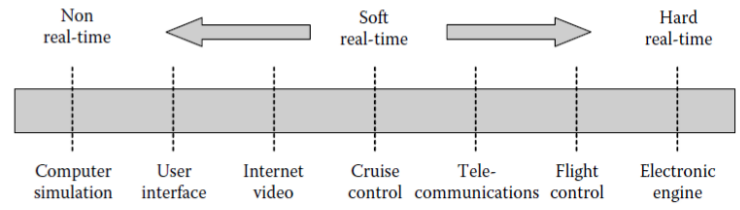
\includegraphics[width=0.7\linewidth]{img/realtime.png}
\end{center}

\subsection{Real-Time Tasks}
\begin{description}
    \item[Periodic:] Must be executed with fixed interarrival time
    \item[Sporadic:] Have known minimum interarrival time
    \item[Aperiodic:] No known interarrival time
\end{description}

\subsection{Wireless Sensor Networks}

Wireless Sensor Networks are composed of node (\textit{mote}) used for
monitoring and they communicates with each other and/or a remote server.

\subsubsection{Resource Constraint}
\begin{itemize}
    \item \textbf{Power}
        \begin{itemize}
            \item Batteries and Energy Harvesting
            \item Turn off idle devices
            \item Requires efficient OS and applications
            \item Reduce communication
        \end{itemize}

        \textit{Duty cycle} is the percentage of one period in which a
        signal or system active $\rightarrow$ isolated node will have
        high duty cycle

    \item \textbf{Bandwidth}
    \item \textbf{Memory}: just a few kBytes
    \item \textbf{CPU}: a few MHz
    \item \textbf{Data Transmission}: not enough power to reach server
        directly $\Rightarrow$ Multihop wireless Network
        \begin{itemize}
            \item Dynamic routing
            \item Self-Organizing Networks
        \end{itemize}
    \item Security: Not enough resources for sophisticated intrusion detection,
        encryption.
    \item Hardware: optimized
    \item \textbf{Reliable Data Flow}: Use 2-bit error correction and
        3-bit error detection.
        \begin{itemize}
            \item Store packet at source in circular buffer on flash 
            \item Remove data from source flash when End2End ack. (There
                is also data link ack)
        \end{itemize}
\end{itemize}

IoT = network of physical objects equipped with electronics and network
connectivity that can be sensed and controlled remotely.

\section{Operating Systems}

\subsection{Hardware}

\begin{description}
    \item[Microcontroller Unit]: Contains 
        \begin{itemize}
            \item CPU
            \item Memory (RAM and non-volatile)
            \item Interfaces to sensors and actuators
            \item Communication interfaces and interfaces to external memory
        \end{itemize}

    \item[JTAG] (Joint test action group): Allows to write code and data
        into flash memory or RAM of the MCU without using one of the
        communication interface
    \item[BSL] (Bootstrap Loader): similar JTAG but from a serial interface

        \begin{itemize}
            \item Can be used to debbuging code on the MCU from a PC
            \item Can upload code/data to the memory without any OS or program
                running.
        \end{itemize}

    \item[$\Rightarrow$] JTAG/BSL are useful for completely empty
        device where we can upload code/data without any OS.

    \item[Transceiver] Used to send data and receive data 
    \item[Interfaces and Sensors] Interfaces to sensor/Actuators
\end{description}

\subsection{Interrupts}
In order to make a software that react to the physical world two strategy:

\begin{description}
    \item[Polling] Read status of I/O every few milliseconds $\to$ waste of
        energy because CPU always busy

    \item[Interrupts] Signal to processor that current code execution should be interrupted
        because something important has happened.
        \begin{itemize}
            \item CPU stops execution and jumps to a specific place in the code that is 
                responsible for handling the interrupt
            \item Exist in all CPUs
            \item Handle by OS and device drivers
            \item Interrupts are expensive because of \textbf{context switching}
        \end{itemize} 
\end{description}

\subsection{OS for embedded systems}
OS are not necessary needed but they free the programmer from some concerns
\begin{itemize}
    \item Handle interrupts (events triggered when something happens)
    \item Manage memory
    \item Write your own process scheduler if you need multi-processing for
        background task
\end{itemize}

\paragraph{Linux}
Linux can be used for embedded systems but
\begin{itemize}
    \item requires enough memory 
    \item preemptive scheduling leads to latency for user code as
        kernel code cannot be preempted
\end{itemize}

\subsection{Real-Time OS}
OS specifically designed for real-time systems:
\begin{itemize}
    \item Much smaller than desktop/server OS
    \item Reduced set of functionality
    \item Fast context switch
    \item Guaranteed time-bounded response to interrupts
    \item Tries to avoid code that cannot be preempted
\end{itemize}

\subsection{OSs for WSN}
\begin{itemize}
    \item Thin abstraction layer to hardware(I/O, timers, \ldots)
    \item Limited multiprocessing
    \item Specific network protocol implementations
    \item Power saving
\end{itemize}

\subsubsection{TinyOS}
TinyOS applications consist of components that you can use in your own
application (as a \textit{set of libraries}). Each component is provided
with an interfaces defining the commands (function) and event available
in the component.

\begin{itemize}
    \item The device sleeps most of the time and they wake up when
        an event is triggered.
    \item Event-handling function execute and then device goes back to sleep.
\end{itemize}

\paragraph{Task}
Tasks are functions that can be preempted by interrupts but not by other tasks.
\begin{itemize}
    \item Task scheduler is a FIFO queue
    \item Not possible to post the same task while it is in the queue
    \item Device sleeps when task queue is empty and no event to process
\end{itemize}

\paragraph{Synchronous vs Asynchronous}
Hardware events can happen at any time and interrupt the current execution.
This can result in race conditions for variables shared between hardware and
task.
Compile differentiates between
\begin{itemize}
    \item Synchronous code: reachable only from tasks
    \item Asynchronous code: reachable from interrupts
\end{itemize}

Static analysis allows compiler to detect race conditions so programmer
are forced to explicitly use atomic section.

\paragraph{Optimization}
\begin{itemize}
    \item TinyOS programmed in NesC (subset of C)$\to$ No pointers or 
        dynamic allocation.
    \item Static analysis is used for optimization $\to$ can reduce apps by 60\%
\end{itemize}

\subsubsection{Contiki}
Differences with TinyOS
\begin{itemize}
    \item No special description language
    \item Cooperative process instead of task queue
    \item Core (kernal + libraries) is uploaded once
    \item Applications can be loaded at run-time
\end{itemize}
Application are composed of one or multiple processes. Proccesses are
cooperative, meaning that other processes can only run if current process
stops.
\begin{itemize}
    \item Processes communicate with each other by posting event
        \begin{itemize}
            \item Synchronous events: delivered immediately
            \item Asynchronous events: delivered later
        \end{itemize}
    \item Processes implemented as Proto-Threads
        \begin{itemize}
            \item Like threads but cheaper
            \item No separate stack per process $\to$ Local variables lose
                their value after a context switch
        \end{itemize}
    \item Process can be preempted by interrupts triggerd by hardware events.
\end{itemize}
\subsubsection{RIOT}
RIOT application programmed in C or C++ and used Multi-threading 
(not event-driven). $\to$ Use priority based scheduling.

\subsection{Networking Stacks}
uIP : Ipv4 stack in 4-5 KBytes of code.
\begin{itemize}
    \item One single packet buffer $\to$ easier to manage
    \item Incoming packet must be processed immediately $\to$ Radio interface queue
        incoming packet while processing.
    \item Retransmission is left to the application to recreate lost
        packet segments (not too bad if we considerer that packet
        contained sensor data, in this case new data are sent)
    \item Send segment one at the time, wait ACK before sending next segment

        $\Rightarrow$ saves memory, simplifies implementation but
        affects performance
    \item One single buffer for IP fragment reassembly
\end{itemize}


\section{TinyDB}
%%TODO


\section{Real-Time Scheduling}
\begin{description}
    \item[Job/processes/threads]: A task to be executed which compete for
        limited resource, the CPU
    \item[Scheduling:] Given N jobs, in which order should the CPU execute
        them
\end{description}

\paragraph{Scheduling goals}:

\begin{tabular}{lm{0.45\linewidth}m{0.45\linewidth}}
    & In general purposes OS( Linux,Windows, \ldots) &
    Real-time OS \\
    &
    \begin{description}
        \item[Fairness] All jobs should be finally executed (no starvation)
        \item[Optimize response time] Should be as short as possible on average
        \item[Optimize throughput] serve as many jobs as possible on average
            (Time to wait for CPU + Execution Time)
    \end{description}
    &
    In real-time system it's a bit different, the 
    \begin{itemize}
        \item most important thing is that task meets their deadline
        \item Don't care about fairness and throughput
        \item Focus on worst-case performance instead of average performance
    \end{itemize}
\end{tabular}

\subsection{Scheduling in general purpose OS}
Based on the idea of Round Robin scheduling which is preemptive with time
slice:
\begin{enumerate}
    \item All jobs wait in a queue for the CPU
    \item Job at the head of the queue receives service for time quantum Q
    \item Then it is interrupted by the next waiting job and goes back to the
        end of the queue
    \item Repeated until job is finished
    \item If Q is small, illusion of parallelism but careful of the cost for
        context switching
\end{enumerate}
By default all jobs are equal: order in queue is order of arrival and same time
slice for all jobs. But there are some variation with different priority and 
different time slice. Priority can be assigned manually or automatically

\subsection{Schedulability in real-time}
\begin{itemize}
    \item Given a set of tasks with their periods, deadlines, etc.
    \item Given a scheduling algorithm
    \item[$\Rightarrow$] The task set is \textbf{schedulable} if all jobs meet their deadlines.
\end{itemize}

Ways to know if task set is schedulable:
\begin{tabular}{l}
    Measurement on real system : expensive!\\
    Simulation\\
    \textcolor{red}{Mathematical analysis}\\
\end{tabular}

\paragraph{Assumption}
\begin{itemize}
    \item Single CPU
    \item No priority inversion
    \item Zero overhead for context switching
    \item Fixed number $N$ of independent periodic tasks with
        period $T_i$ and deadline $D_i$ (relative to begin of period), $i$=1,\ldots, $N$
    \item Task $i$ has a worst-case execution time $C_i$
\end{itemize}

\subsubsection{Rate Monotonic Scheduling}

RM is on \textcolor{red}{optimal} preemptive static priority scheduling
algorithm. It assigns a static priority to each task, the task with the shortest period
has highest priority. Preemption is possible.
\newline

Assuming $D_i=T_i$ for all tasks, a sufficient (but too pessimistic) test 
for schedulability with RM is:
$$\sum_{i=1}^N \frac{C_i}{T_i}\leq N(2^{\frac{1}{N}}-1)$$

\begin{center}
    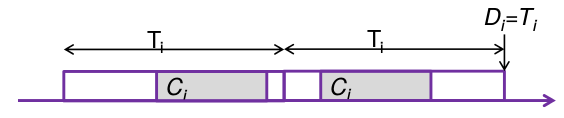
\includegraphics[width=0.5\linewidth]{img/RM.png}
\end{center}

RM is easy to implement with low overhead since task priorities are set at 
design time and does not change during run time but RM does not 
allow high CPU utilization because scheduling too rigid

\paragraph{Worst Case Execution Time}
To know worst case execution we can either do measurement or use static analysis

\subsubsection{Deadline Monotonic Scheduling}

RM does is not good for $D_i < T_i$, so in DM, task with shortest deadline
has highest priority. DM is on \textcolor{red}{optimal} preemptive static priority scheduling
algorithm for $D_i<T_i$.
$$\sum_{i=1}^N \frac{C_i}{D_i}\leq N(2^{\frac{1}{N}}-1)$$

\begin{center}
    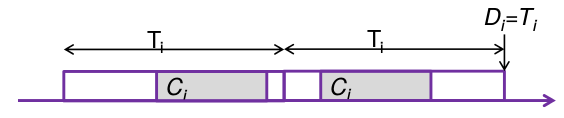
\includegraphics[width=0.5\linewidth]{img/RM.png}
\end{center}

\subsubsection{Response Time Analysis}
RTA provides a sufficient and necessary test for all fixed-priority preemptive 
scheduling algorithms (RM,DM,\ldots)\\
A task set is schedulable if worst-case response time $R_i \leq D_i$ for all tasks.
\begin{itemize}
    \item Response time $R_i$ = $C_i + I_i$ where $I_i$ is the worst
        case interference time = amount of time a task is delayed by
        execution of higher priority tasks
\end{itemize}

\begin{eqnarray}
    R_i =& C_i + I_i\\
    R_i =& C_i + \sum_{j\in hp(i)} \lceil \frac{R_i}{T_j}\rceil C_j
    \label{rta-eq}
\end{eqnarray}

where hp(i) is the set of tasks with higher priotity than task i 
$\to \lceil \frac{R_i}{T_j}\rceil$ is the number of preemptions of task i by task j.



~\eqref{rta-eq} is a recursive formula so it is solve by finding smallest fixed point:
$$R_i^0 = C_i$$
$$R_i^{m+1} = C_i + \sum_{j \in hp(i)} \lceil \frac{R_i^m}{T_j}\rceil C_j$$

\subsubsection{Earliest Deadline First}

Optimal preemptive \textbf{dynamic} priority scheduling algorithm 
where task with earliest absolute deadline has the highest priority. The
absolute deadline is the time when the job is ready + $D_i$.

\subsection{Scheduling with resource lock}

We have assumed that task are independent, in a real systems, tasks can
be dependent because they access a shared resource in a critical section
(CS). In this case, a task with highest priority can be
\textbf{unboundedly} blocked by tasks with lower priority. Response time
becomes: $$R_i = C_i + I_i + B_i$$ where $B_i$ is the time the task is
blocked because a resource has been locked.

\begin{center}
    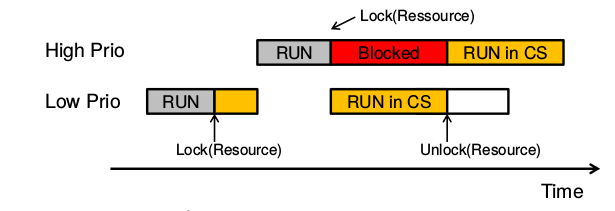
\includegraphics[width=0.5\linewidth]{img/priority.png}
\end{center}

\paragraph{Note:} RTA a test only sufficient, not necessary with blocking.

\paragraph{Priority inversion problem}

\begin{center}
    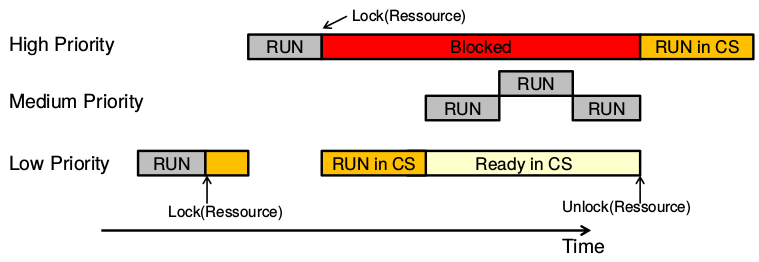
\includegraphics[width=0.5\linewidth]{img/inversion.png}
\end{center}

\subsubsection{Priority Inheritance Protocol}

To avoid this problem, a low-priority task inherits the priority of the 
blocked high-priority task.
\begin{itemize}
    \item When task i is blocked by a CS held by task k 
        and prio(i) > prio(k) $\to$ prio(k) := prio(i)
    \item When task k leaves the CS:
        \begin{itemize}
            \item If task k no longer blocks any tasks, it returns to its old priority
            \item If task k still blocks other tasks, it inherits their highest priority
        \end{itemize}
\end{itemize}

\subsubsection{Priority Ceiling Protocol}
Alternative to priority inheritance, a shared resource R can be accessed
only tasks $S_R = \{ t_1,\ldots,t_m\}$.
\begin{itemize}
    \item Assign a priority ceiling $C_R$ to that resource
        $$C_R = max_{t_i\in S}(prio(t_i))$$
    \item When a task locks that resource, its priority is immediately
        boosted to $C_R$
\end{itemize}

\paragraph{Note:}
Priority inheritance and priority ceiling require a scheduler that can handle
dynamic priorities

\subsection{Aperiodic/sporadic tasks}

\begin{itemize}
    \item \textbf{With hard deadlines}
        \begin{enumerate}
            \item \begin{itemize}
                    \item Take the lowest inter-arrival time L of those tasks
                    \item Treat them as a virtual periodic task with period L in 
                        schedulability analysis
                    \item[$\Rightarrow$]Too pessimistic
                \end{itemize}
        \end{enumerate} 

    \item \textbf{Without hard deadlines}
        \begin{enumerate}
            \item \begin{itemize}
                    \item Maintain the hard deadlines for the periodic tasks
                    \item Try to reduce response time for the other tasks
                \end{itemize}

                Simple and no impact on periodic tasks but possibly very
                long response times if the system is very busy with
                periodic task

            \item Polling server
                \begin{itemize}
                    \item A periodic task (''server'') with period $T_S$ to serve 
                        aperiodic/sporadic requests
                    \item Incoming aperiodic/sporadic jobs are queued in a queue
                    \item In one execution period, the server only runs up to $C_S$ time units
                \end{itemize}
                Performance can be controlled by the period and the priority of the server
                tasks and by $C_S$. 

                \begin{itemize}
                    \item Advantage: Polling server can be treated like a periodic task with
                        WCET $C_S$
                    \item Disadvantage: If an aperiodic/sporadic job is not handled by the
                        server in a time period, it has to wait for the next period $\to$ 
                        response time increases
                    \item Can be extended to multiple servers with different priorities,
                        periods and $C_S$ for different classes/types jobs.
                \end{itemize}
        \end{enumerate}
\end{itemize}


\section{Wireless Communication}

\begin{tabular}{|l|ccc|}
    \hline
    Classification & Mobile & Wireless Sensor Network & Internet Of Things\\
    \hline
    Network size & Millions & Thousand & Millions to Billions? \\
    Range & 100 to 1000$km^2$ & $m^2$ to $km^2$ & $m^2$ to $km^2$\\
    Mobility & Mobile & Static or mobile & Static or mobile \\
    Roaming & Yes & x & x \\
    Energy & Not critical & Critical & x \\
    Speed & Best without constraint & x & x \\
    \hline
\end{tabular}


\subsection{Radio spectrum}
Not all frequencies are equally suitable for all purpose
\begin{itemize}
    \item $\neq$ propagation properties
    \item $\neq$ power emission
    \item Some a reserved (police, phone) other are license free
\end{itemize}

\subsection{Path loss}

Signal strength is attenuated as the electromagnetic wave propagates
through space.

\subsubsection{Free-space loss}
Attenuation depends on frequency and distance
$$\frac{P_r}{P_t} = G_t \times G_r \times ( \frac{\lambda}{4\pi R})^2$$
where \begin{tabular}{rl}
    $P_r,P_t$ & is the received and transmitted power\\
    $G_r,G_t$ & is the received and transmitted antenna gain\\
    $R$ & is the distance between transmitter and receiver\\
    $\lambda$ & is the wave length\\
\end{tabular}

$$PL[dB] = 10 log\frac{P_t}{P_r} = - 10 log\frac{P_r}{P_t}$$

\subsubsection{Others loss}
\begin{center}
    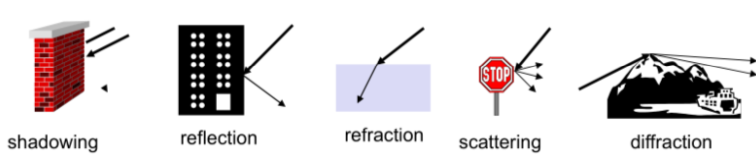
\includegraphics[width=0.7\linewidth]{img/loss.png}
\end{center}

\begin{itemize}
    \item Reflection and refraction depend on material and wave
        length
    \item Multi-path (scattering, diffraction,...)
        $$\frac{P_r}{P_t} = G_t \times G_r \times ( \frac{\lambda}{4\pi
        R})^\gamma$$
        where $\gamma$ is 3-5 in cities, 4-6 in buildings,...
    \item Noise due to
        \begin{itemize}
            \item Receiver electronics
            \item Interference on wireless channel:
                B far away to be detected by A, but still causes
                interference in form of background noise.
                \begin{center}
                    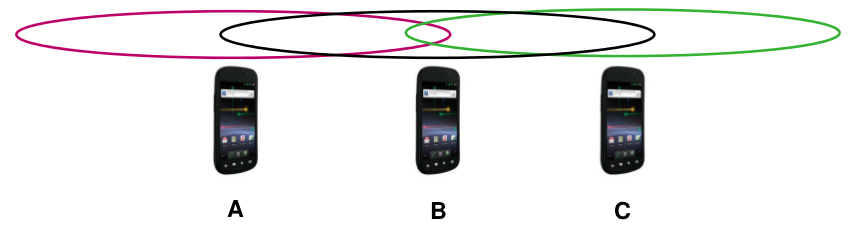
\includegraphics[width=0.5\linewidth]{img/ranges.png}
                \end{center}

                \paragraph{Hidden stations}: (1) C cannot detect A, (2) send data to B
                but (3) B cannot receive because A is sending
                \paragraph{Far stations}: (1) A is closer to B than C so
                (2) signal of A so strong that B cannot receive C
        \end{itemize}

        Stronger the noise, harder for the receiver to interpret signal
        as a symbol ($0-1$).
        \begin{itemize}
            \item Expressed as Signal-To-Noise: $$SNIR = 10 log(\frac{P_r}{N_0 + \sum_j I_j})$$ 
                where \begin{tabular}{rl} $P_r$ & Received signal power \\
                $N_0$ & Noise power \\
                $I_j$ & Influence of interfering neighbor $j$
            \end{tabular}

        \item With an appropriate Medium Access protocol (we will see
            that later), interference can be reduced. SNIR simplifies to
            SNR (Signal-Noise-Ratio)
            $$SNR=10 log(\frac{P_r}{P_N})$$
            where \begin{tabular}{rl} $P_r$ & Received signal power \\
            $P_N$ & noise power varies from locality\\
        \end{tabular}
\end{itemize}
\end{itemize}

\subsubsection{Error Rate} 
\begin{itemize}
    \item BER (Bit Error Rate): Number of bit errors per time unit
        $\Rightarrow$ depends on $SNR$

        $p_b$ is the probability that a received bit will be in error
    \item PER (Packet Error Rate): Packet rate error.
        $p_p$ is the probability that a received packet has an error
\end{itemize}

$$p_p = 1 - (1 - p_b)^N$$ where $N$ is the packet size


\subsection{Physical layer}

%\begin{center}
%    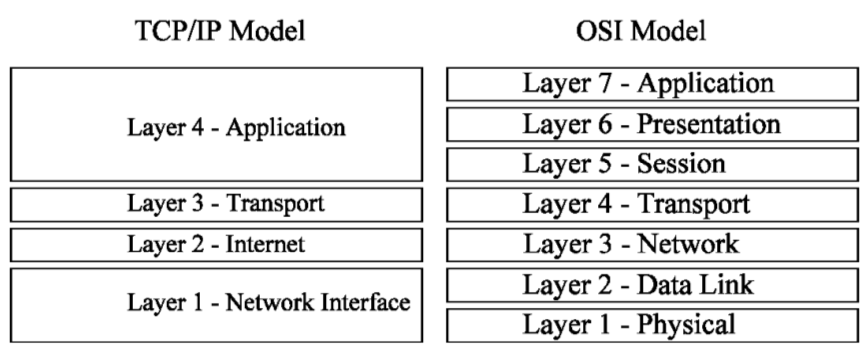
\includegraphics[width=0.6\linewidth]{img/osi.png}
%\end{center}
\begin{center}
    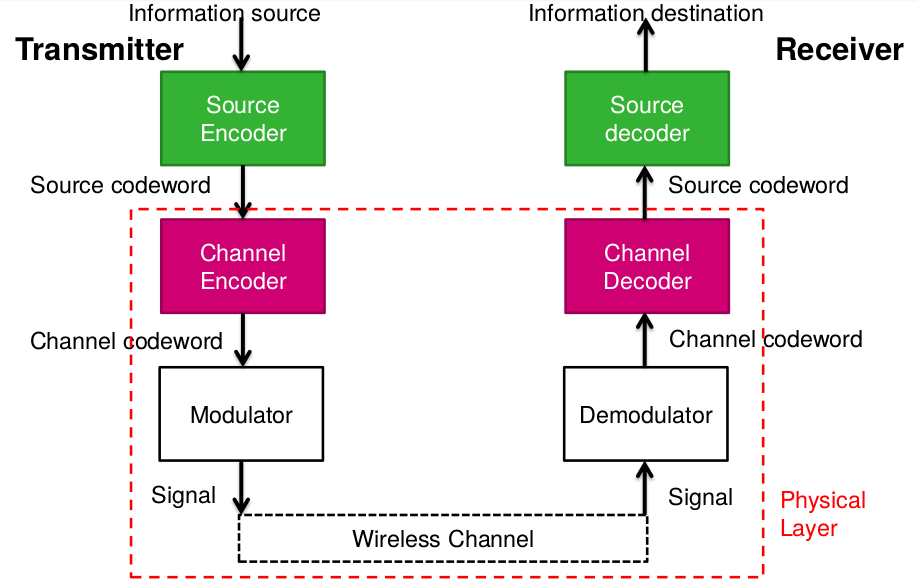
\includegraphics[width=0.8\linewidth]{img/physical.png}
\end{center}

\subsubsection{Channel encoding}
\begin{itemize}
    \item Add error detection code to the data (parity bits, CRC)
    \item Block coding 

    \item interleaving (shuffle symbols): As electromagnetic spikes can
        cause burst errors, many errors in one code word $\Rightarrow$
        exceeds error-correcting capabilities.

        Shuffle symbols to distribute error over several words: Hello
        World $\rightarrow$ HWeol rllod
\end{itemize}

\subsubsection{Modulation}
Radio wave as sine function: $signal(t) = A \times sin(2\pi \times t
\times f + \phi)$ with Amplitude (A), Frequency (f) and Phase ($\phi$).


Modulation manipulates these parameters as a function of time to
transmit data.
\begin{center}
    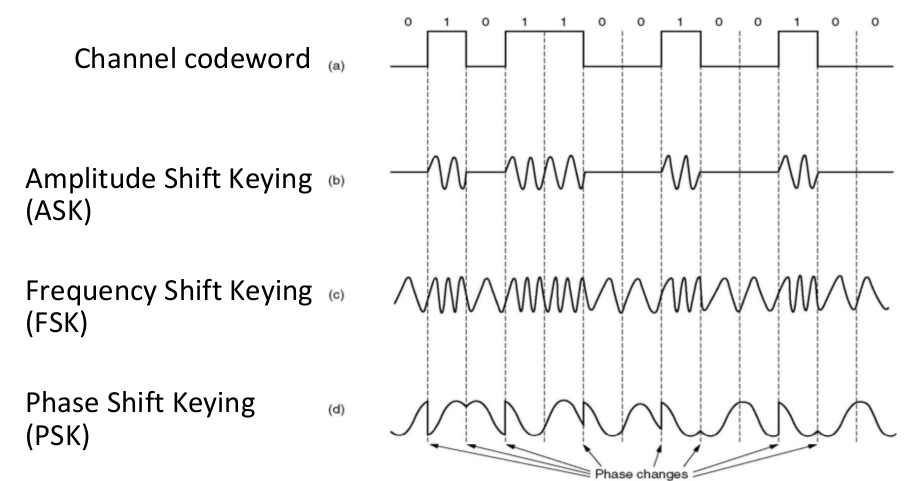
\includegraphics[width=0.6\linewidth]{img/modulation.png}
\end{center}

Challenge: bit synchronization, frame synchronization, listing same
frequency, noise, interference,...


\section{Medium access}

Control medium access, but allow concurrent medium usage $\Rightarrow$
multiplexing.

\begin{table}[!h]
    \begin{tabular}{|r|cccc|}
        \hline
        & SDMA & FDMA & TDMA & CDMA \\
        \hline
        Coordination & None & Frequency assignment & Time synchronization & Code coordinations \\
        Viable & x & x & v & v \\
        \hline
    \end{tabular}
\end{table}

\begin{itemize}
    \item \textbf{Space Division Multiple Access (SDMA)}: divide space
        so that devices do not interfere.
        \begin{center}
            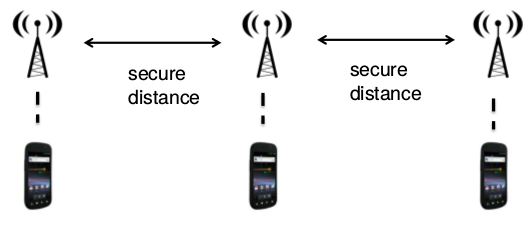
\includegraphics[width=0.6\linewidth]{img/SDMA.png}
        \end{center}

        \begin{itemize}
            \item Simple, but pure SDMA require huge secure distance and one
                station per end point: not viable in practice without other
                multiplex methods!
        \end{itemize}

    \item \textbf{Frequency Division Multiple Access (FDMA)}:
        Frequencies permanently assigned to transmission channels
        \begin{center}
            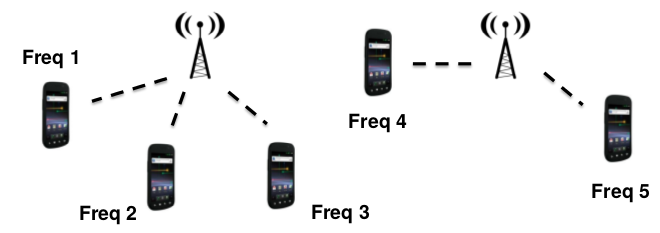
\includegraphics[width=0.6\linewidth]{img/FDMA.png}
        \end{center}

        \begin{itemize}
            \item One frequency per station and these frequency require
                \textit{guard-bands} between them such that they are more robust
                against interferences
        \end{itemize}
        \begin{center}
            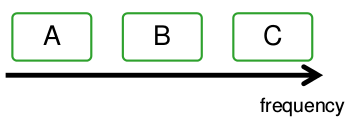
\includegraphics[width=0.3\linewidth]{img/guard.png}
        \end{center}

    \item \textbf{Time Division Multiple Access (TDMA)}:
        Time is divided into slots and only one station per slot can
        access medium
        \begin{center}
            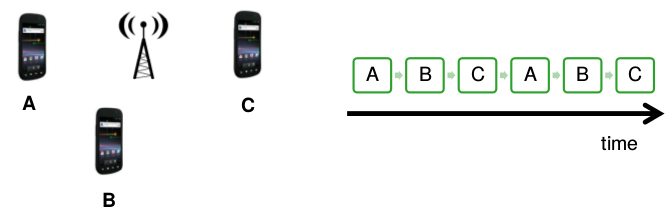
\includegraphics[width=0.6\linewidth]{img/TDMA.png}
        \end{center}

        \begin{itemize}
            \item One frequency, time division can be done in
                control software 
            \item but $\Rightarrow$ Require \textbf{exact timing} between stations
                (use \textit{guard-times} between slots to be more tolerant
                against timing variations)
        \end{itemize}

    \item \textbf{Code Division Multiple Access (CDMA)}: Each sender
        uses a different code that is applied to the data stream and if
        receiver know the code it can decode the data.

        \begin{enumerate}
            \item Sender A: \begin{tabular}{l} send bit=1\\
                Code=010011\\ Ouput = (-1 +1 -1 -1 +1 +1)\end{tabular}
            \item Sender B: \begin{tabular}{l} send bit=0\\
                Code=110101\\ Ouput = (-1 -1 +1 -1 +1 -1)\end{tabular}
            \item superimposed: (-2 0 0 -2 +2 0)
            \item Extract A: (-2 0 0 -2 +2 0) * (-1 +1 -1 -1 +1 +1) = 6
                $\geq$ 0 $\Rightarrow$ original bit is 1
        \end{enumerate}

        \begin{itemize}
            \item Need much longer codes which needs more bandwidth than
                original. 
            \item Coordination between station to have different code or
                stations choose code randomly
            \item Senders have to adapt their transmission power to all have
                the same strength at a receiver
        \end{itemize}
\end{itemize}

\subsection{Assignment}







\section{Routing with RPL}
\subsection{Routing Protocols}
There are two classes of routing protocols:
\begin{itemize}
	\item Link-State: Each node knows network topologu and runs a shortest-path 
	algorithm $\to$ powerful but require more resources
	\item Distance-Vector: a node only needs to know which neighbor leads
	to which node.
	\begin{itemize}
		\item Each node maintains for each destination, the minimum distance
		and the neighbor to forward to.
	\end{itemize}
\end{itemize}
\paragraph{Count To Infinity problem with DSV routing}
\begin{figure}[ht!]
	\centering
	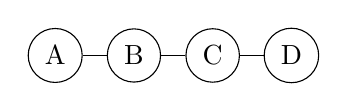
\begin{tikzpicture}
		\node[shape=circle,draw](a){A};
		\node[shape=circle,draw,right of=a](b){B};
		\node[shape=circle,draw,right of=b](c){C};
		\node[shape=circle,draw,right of=c](d){D};
	
		\draw[-] (a) -- (b);
		\draw[-] (b) -- (c);
		\draw[-] (c) -- (d);
	\end{tikzpicture}
	\caption{Count-To-Infinity, distance metric: number of hops}
\end{figure}
\begin{itemize}
	\item Initial state: B knows that A is 1 hop away
	\item A disappears. B removes it from its routing table
	\item Before B notifies C, C sends that A is 2 hop away to B
	\item B thinks it has found a new path to A, so it store this path
	and send that A is 3 hop-away
	\item C update its routing table A is 4 hop away and sends
	\item \ldots
\end{itemize}

\subsection{RPL}
RPL is a routing protocol designed for Low-power and Lossy Networks (LLN).
Characteristics of such networks:
\begin{itemize}
	\item Lossy,slow and unstable links
	\item Traffic mostly flows form devices to a server/sink or border
	router( or in opposite direction)
	\item Large number of nodes
	\item Constrained devices with small memory
\end{itemize}
\subsubsection{Routing Topology}
Topology represented as a Destination Oriented Directed Acyclic Graph (DODAG)
where the root is a server, border router, etc.
\begin{figure}[ht!]
	\centering
	\begin{tikzpicture}
		\node[shape=circle,draw,fill=green](root){0};
		\node[shape=circle,draw,below left of=root](c1){1};
		\node[shape=circle,draw,below right of=root](c2){1};
		\node[shape=circle,draw,below left of=c2](c3){2};
		\node[shape=circle,draw,below right of=c3](c4){3};
		\node[shape=circle,draw,below left of=c3](c5){3};
		
		\node[left =1cm of root](ds){};
		\node[below =2cm of ds](de){};
		
		\node[right =1cm of root](us){};
		\node[below =2cm of us](ue){};
		
		\draw[->] (c1) -- (root);
		\draw[->] (c2) -- (root);
		\draw[->] (c3) -- (c1);
		\draw[->] (c3) -- (c2);
		\draw[->] (c4) -- (c3);
		\draw[->] (c5) -- (c3);
		\draw[->] (c4) -- (c2);
		\draw[->] (c5) -- (c1);
		
		\draw[->] (ds) -- (de);
		\draw[->] (ue) -- (us);
	\end{tikzpicture}
	\caption{root in green, number correspond to node rank}
\end{figure}
\begin{itemize}
	\item Not a tree as they are multiple path possible for a destination.
	\item An RPL is a set disjoint DODAGS
	\item You can have multiple RPL instances on the same physical network
	\item Each RPL control messages carry a DODAG ID and a RPL-instance ID
	\item Rank is node property, typicallt proportional to path cost but coarser.
	The rank of node must be greater than rank of parent.
\end{itemize}
\subsubsection{RPL Control Messages}
\paragraph{DAG Information Object (DIO)}
\begin{itemize}
	\item Link-local multicasted by existing RPL nodes to advertise a DODAG
	\item Sent periodically by but also on request when routing problem detected
	\item Contains rank od sending node and network prefix
	\item Nodes find parent(s) in this way
	\item Multiple parents possible. Choice depends on path costs
\end{itemize}
$\Rightarrow$ Nodes know about possible parents and routes up toward DODAG root
established.
\subparagraph{Version Number}
When the root advertises a DODAG with the DIO message, it also includes a version
number
\begin{itemize}
	\item A that joins a DODAG with version X ignores lower versions
	\item When a node receives a message with higher version, it can move to that 
	version $\to$ new rank and parent
\end{itemize}
The root can decide to increase the version number and advertise a new version
of the DODAG. It typically happens when a problem with current DODAG is 
detected and there is a repair.
\subparagraph{Path Cost}
To compute how expensive a path is, the DODAG can define a Objective
Function that the nodes must used. Cost can expressed in terms of:
\begin{itemize}
	\item Signal quality
	\item Throughput
	\item Delay
\end{itemize}

\paragraph{Destination Advertisement Object}
\begin{itemize}
	\item DAO messages travel up and forwarded to root
	\item Are unicasted to parent (or link-local multcasted to help for 
	direct P2P traffic)
	\item The goal is to propagate information about children(new and disappeared)
	 so that parents can populate their routing table.
\end{itemize}
$\Rightarrow$ Routes down away from root established

\paragraph{DODAG Information Solicitation (DIS)}
Node send DIS message to request DIO when:
\begin{itemize}
	\item A new node want to joins an RPL instance
	\item A sleeping node wakes up and needs recent information
	about the network or want to inform the network that it is back
	\item A node cannot reach the router anymore $\to$ looking
	for a new parent
\end{itemize}
\subsection{Packet Forwarding}
\begin{itemize}
	\item In up direction:
	\begin{itemize}
		\item Packet is sent to lower rank (or siblings, if no lower rank)
	\end{itemize}
	\item In down direction
	\begin{itemize}
		\item Node knows route to destination thanks to DAO message
	\end{itemize}
\end{itemize}
Node only store information about next hop to destination, it's a DSV
with ranks.

\subsubsection{Loop Avoidance Mechanism}
\paragraph{IPv6 header option}
There is a direction flag in the header indicating the expected direction
of a data packet:
\begin{itemize}
	\item Sender sets the direction
	\item If an up-packet is forwarded from a node A to a node B with 
	higher rank, a problem is detected by B (same in opposed situation)
	\item Node B sets the R (repair flag) in the packet. This indicates
	that the DODAG has to be repaired
\end{itemize}

\paragraph{Node movement}
Node might find better parents:
\begin{itemize}
	\item New nodes appear or old nodes disappear
	\item Signal strength changes
\end{itemize}
However, node are only allowed to move up toward the root $\Rightarrow$ A node
cannot become a child of one of its children.

\subsubsection{Trickle Timer}
A DIO message are sent to build new DODAG, on a DIS message and periodically. To
avoid that to send to many DIO when it's not necessary, a Trikle Timer is run
on each node:
\begin{itemize}
	\item $T_min$: minimum duration of the timer
	\item $T_max$: maximum duration of the timer
	\item $T$: current duration used by the timer
	\item $C$: number of good messages received by the node
	\item $K$: some threshold for C
\end{itemize}
\begin{lstlisting}[frame=single]
T:= Tmin, C:=0
t = rand(T/2,T)
wait(event)
	if event == t expires and C<K:
		send DIO 
		restart t
	if event == T expires:
		T:= 2*T (up to Tmax)
		restart T
		t := rand (T/2,T)
	if event == good DIO:
		C:= C+1
	if event == bad DIO:
		C:= 0
		T= Tmin
		t:=rand(T/2,T)
\end{lstlisting}
\begin{itemize}
	\item C is increased by 1 for every good message = DIO that does not announce a
	change
	\item C is reset to 0 and T is reset to $T_min$ for bad message= DIO that 
	announces a change or with R flag.
\end{itemize}
Good message indicate a stable network and because T is increased,
nodes send DIS messages less messages less frequently.

\section{Constrained Application Protocol}
An HTTP-inspired protocol designed for constrained devices and networks used
for RESTful access to resources. Default port is 5673 (coap) adn 5684(coaps)\\
Key features:
\begin{itemize}
	\item Low overhead
	\item Easy to implement
	\item For Machine-2-Machine communication
	\item Simple mapping to HTTP for CoAP-HTTP proxies
\end{itemize}
CoAP messages provide reliable messaging over UDP and consist of a set of
method that resemble HTTP request methods and response code.
\begin{figure}[ht!]
	\centering
	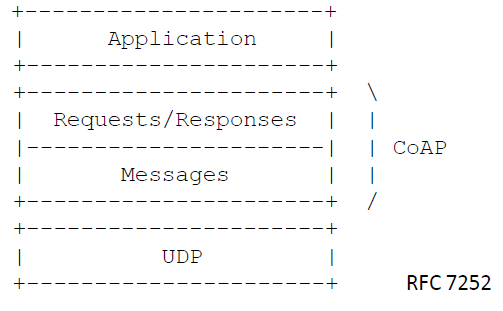
\includegraphics[scale=0.65]{img/coap-layer.png}
\end{figure}
\subsection{Message Format}
Messages are exchanged between UDP end-point and they have the same
format for request and response. Header and options are in binary format.
\begin{figure}[ht!]
	\centering
	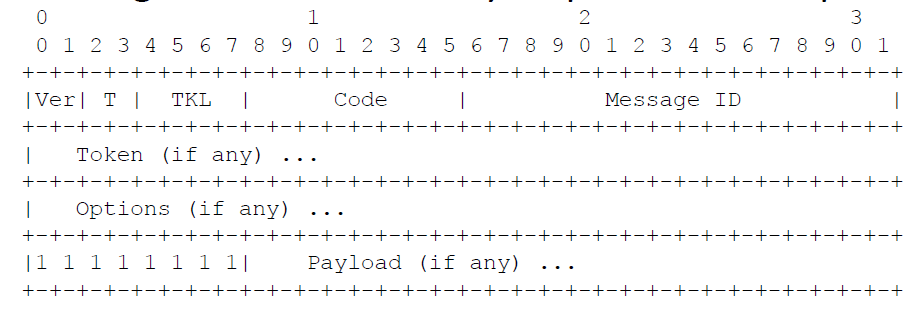
\includegraphics[scale=0.65]{img/coap-format.png}
\end{figure}
Message are compact $\Rightarrow$ avoid IP fragmentation and easy parsing.
\subsubsection{Fields}
\begin{description}
	\item[Ver:] Version number(01). Unknown versions are silently ignored.
	\item[Code:] Method Code in request resp. Response Code in responses
	\begin{itemize}
		\item Method similar to HTTP: GET(0.01), POST(0.02),PUT(0.03),DELETE(0.04)
		\item Response codes similar to HTTP responses code: ok (2.05), not found
		(4.04),\ldots
		\item URI and additional options are stored in the options fields.
	\end{itemize}
	
	\item[Options:] Additional (0 or more) options, end marked by 1111111
	\begin{itemize}
		\item Options identified by their option code
		\item Option Code = Delta + previous option code
		\item Option length = length of option in bytes
		\item Delta is used to indicate presence of extension fields
	\end{itemize}
	An URI such as \texttt{coap://example.com:5683/sensors/temp?x=1\&y=2} is not
	stored as one big string in a request but it is store as option.
	\begin{itemize}
		\item Host name in Uri-Host option (code 3)
		\item Port in Uri-Port option (code 7)
		\item Path segments in one or more Uri-Path options (without /)
		\item Query arguments in one or more Uri-Query (without \& and ?)
	\end{itemize}
	$\Rightarrow$ Simplifies parsing.
	
	\item[Token:] A 0 to 8 bytes value (length in TKL) generated by the client
	for concurrent request. Request for same source-dest should have unique token
	number.
	\begin{itemize}
		\item Response will use same number as the request
		\item Responses with unexpected token number are rejected
	\end{itemize}
	CoAp connection can use Datagram Transport Layer Security which is like TLS but
	for UDP. If DTLS is not used , token should be long randomized token value to
	prevent response spoofing.
	
	\item[T:] Specifies the type of the message:
	\begin{itemize}
		\item Confirmable(0)
		\item Non-confirmable(1)
		\item Acknowlegment(2)
		\item Reset(3)
	\end{itemize}
\end{description}

\subsection{Transmission}
Depending on the type of the message, its treatment will be different
\subsubsection{Transmission without Reliability}
Lightweight and useful for repeated operations, it applies to request or response
of type \textcolor{red}{Non-confirmable}.
\begin{itemize}
	\item Message might be sent multiple times by sende or network so each copy
	as a unique message ID to identify them.
	\item Message is ignored by recipient if unexpected or ill-formatted
	(unknonw codes,wrong token value) $\to$ Recipient may send Reset 
	message with same message ID
\end{itemize}
\subsubsection{Transmission with Reliability}
This applies to message of type \textcolor{red}{Confirmable}, Message ID
is crucial but not only for de-duplication. Indeed, recipient must either
reply with:
\begin{itemize}
	\item Acknowledgement (with same message ID) or 
	\item Reset (with same msg ID) and ignore the message
\end{itemize}
Sender retransmits Confirmable message until ACK or Reset received 
(or runs out of attempts)
\paragraph{Retransmission}
Exponential back-off
\begin{lstlisting}[frame=single]
ACK_TIMEOUT = 2s
ACK_RANDOM_FACTOR = 1.5
MAX_RETRANSMIT = 4

timeout := rand(ACK_TIMEOUT,ACK_TIMEOUT*ACK_RANDOM_FACTOR)
retransmission-counter := 0
(*) send CON message
wait until timeout or ACK or RESET
if timeout and retransmission-counter < MAX_RETRANSMIT:
	timeout := timeout*2
	retransmission-counter++
	go to (*)
\end{lstlisting}

\subsubsection{Synchronous Message Exchange}
\begin{minipage}{0.5\textwidth}
	\begin{figure}[H]
		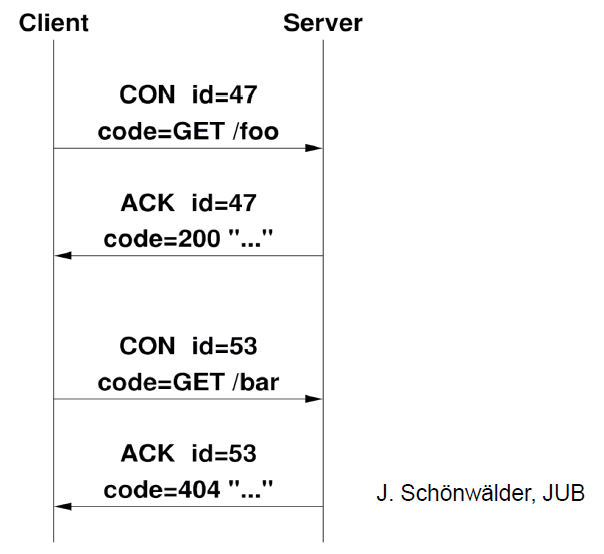
\includegraphics[scale=0.5]{img/syn-exchange.png}
	\end{figure}
\end{minipage} \hfill
\begin{minipage}{0.45\textwidth}
	\begin{itemize}
		\item Request sent as CON message
		\item Response sent as ACK message (piggybacking)
		\item Efficient
	\end{itemize}
\end{minipage}




\subsubsection{Asynchronous Message Exchange}
\begin{minipage}{0.5\textwidth}
	\begin{figure}[H]
		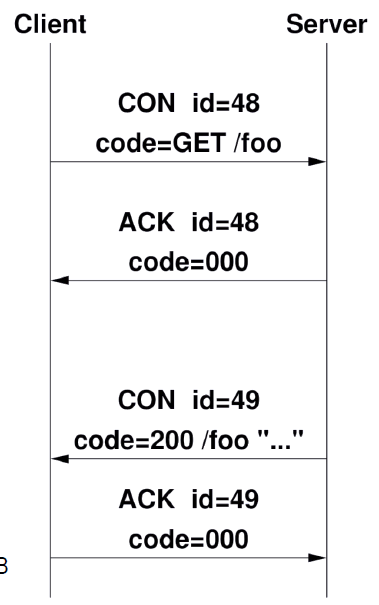
\includegraphics[scale=0.5]{img/asyn-exchange.png}
	\end{figure}
\end{minipage} \hfill
\begin{minipage}{0.45\textwidth}
	\begin{itemize}
		\item Request sent as CON message
		\item Recipient replies immediatel with empty ACK message (code 0.00)
		\item Recipient replies later with actual response in CON message
		\item More overhead than piggybacking
		\item Tokens for matching request <-> response
	\end{itemize}
\end{minipage}

\paragraph{Remarks}
\begin{itemize}
	\item CON and NON-CON messages can be mixed, ex: request as NON-CON and
	response as CON
	\item Empty CON (code 0.00) can be used as ping message, recipient replies with
	RESET message
	\item No definition of how long request should wait for response, CON-ACK 
	mechanism is only about reliable transmission
\end{itemize}

\subsection{CoAP Features}
\subsubsection{Multicastin and Discovery}
CoAP supports requests to IP multicast groups, if a request is multicast, the
behavior will be a bit different:
\begin{itemize}
	\item Servers must not reply RESET to unwanted NON-CON messages 
	$\Rightarrow$ avoid too many error responses
	\item Servers should wait random time before responding request
	$\Rightarrow$ avoid congestion
\end{itemize}
Multicastinf is useful for automatic service discovery in M2M scenarios.
Servers should also support resource discovery:
\begin{itemize}
	\item Client sends \texttt{GET ./well-known/core} to server
	\item Server returns list of resources
\end{itemize}

\subsubsection{Caching}
CoAp uses a simple caching mode with an \textcolor{red}{age} option indicationg
cache lifetime. This useful for proxies to cache information of sleeping nodes
or to reduce network traffic
\paragraph{Optional ETag}
\begin{enumerate}
	\item Server can put an ETag string in response
	\item Client sends ETag when re-requesting a cached resource
	\item Server can respond with 2.03 (valid) if resource has not
	changed
\end{enumerate}
ETag can be used in PUT-requests with If-Match-Option: Only write 
new value if I have latest one $\Rightarrow$ protection against accidental
concurrent overwrites

\subsubsection{Other Features}
\begin{itemize}
	\item Observing resources
	\item Block transfer (specify wanted bytes in request)
\end{itemize}

\subsection{Spoofing Attack}
CoAp runs over UDP, no handshak \& sequence number
\begin{itemize}
	\item Third party can spoof RESET message to disrupt connection
	\item CoAP endpoints can be used for amplication \& reflection 
	attacks against other targets.
\end{itemize}
Security (DTLS) and careful implementation (randome token) can prevent attack
to some degree.

\end{document}
